\mode*

\section{Välj p-uppgift}

\begin{frame}
  \begin{block}{P-uppgifter}
    \begin{itemize}
      \item Finns ett antal att välja mellan.
      \item Välj utefter vad ni tycker låter intressant/roligt/spännande.
      \item Finns extrafiler (data) länkade.
    \end{itemize}
  \end{block}

  \pause

  \begin{remark}
    \begin{itemize}
      \item Får inte välja samma som er labbpartner.
    \end{itemize}
  \end{remark}
\end{frame}

\begin{frame}
  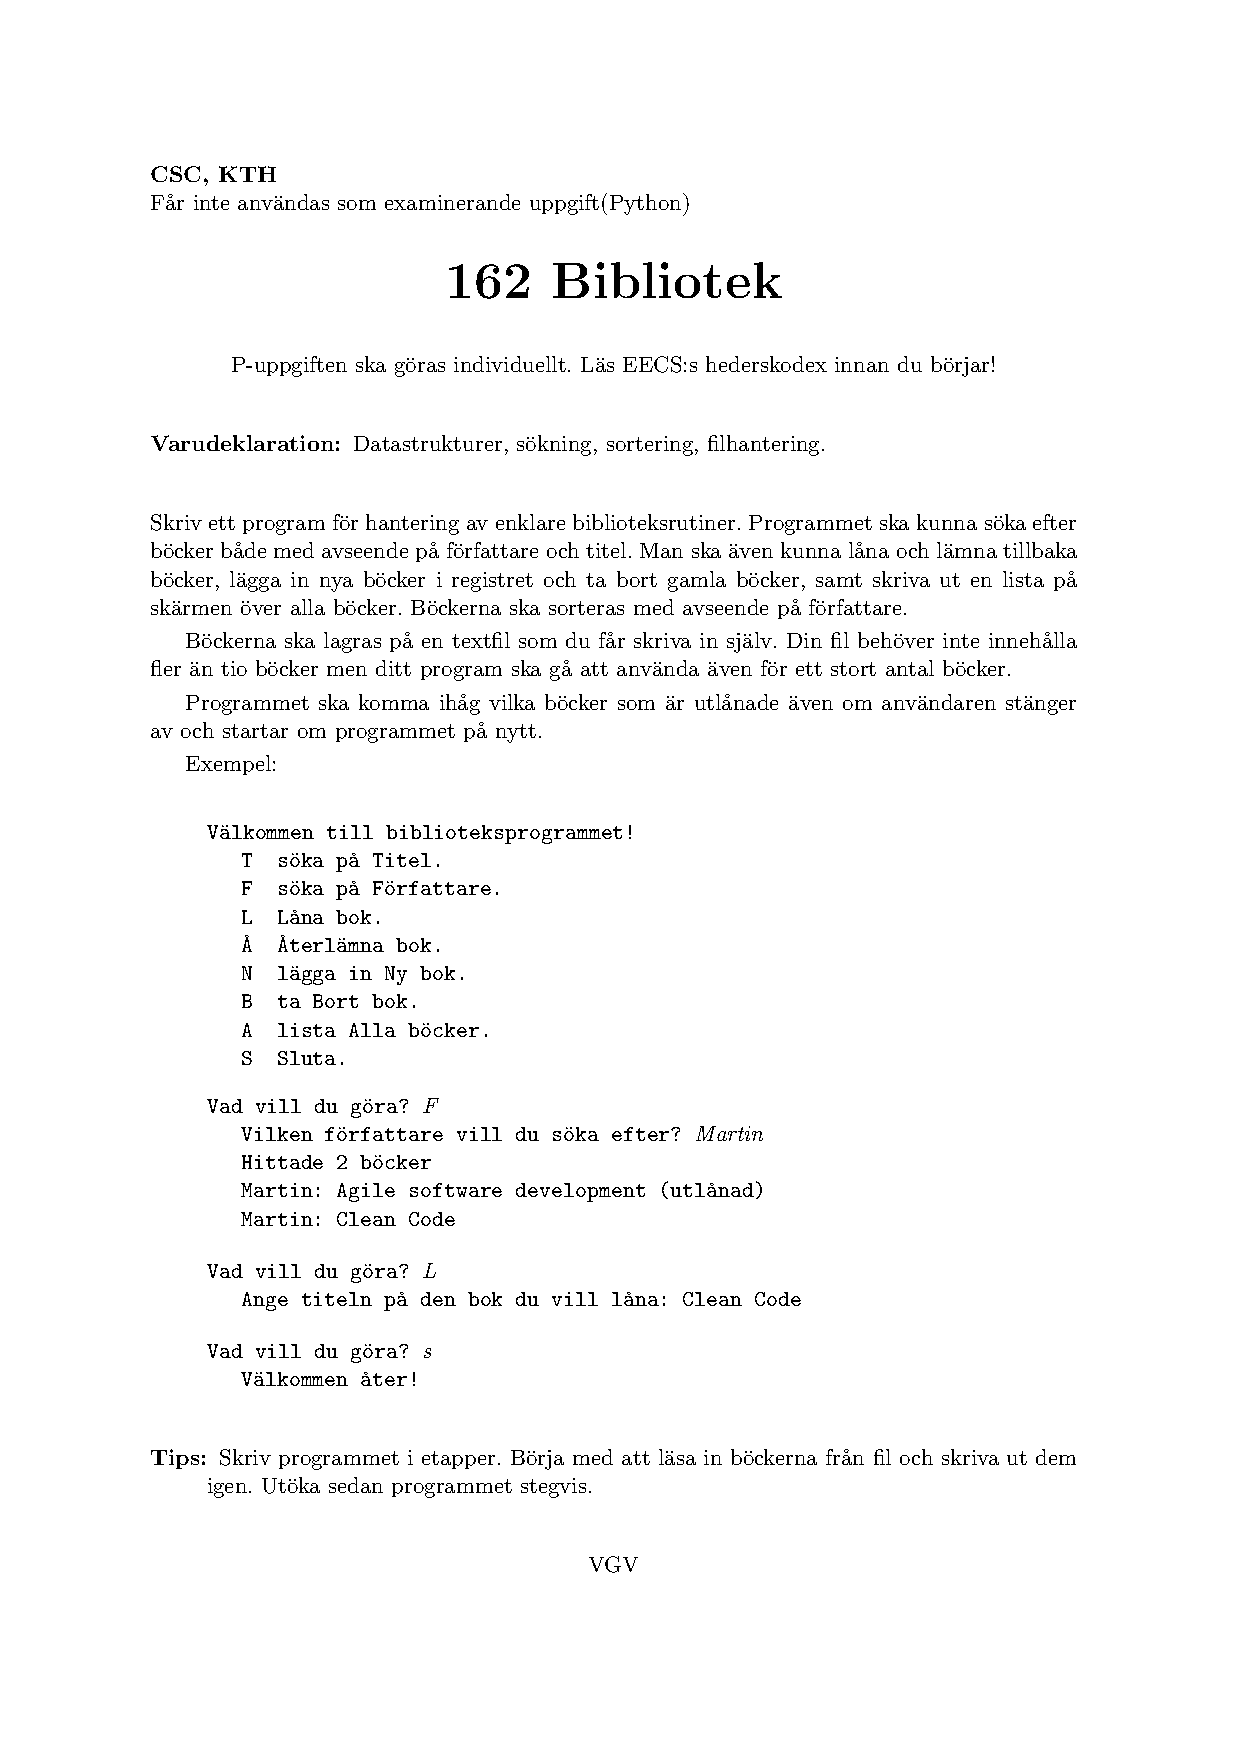
\includegraphics[width=\columnwidth]{exempel.pdf}
\end{frame}


\section{Projektspecifikation}

\begin{frame}
  \begin{block}{Specifikation}
    \begin{description}
      \item[Algoritm] Hur ser algoritmen ut som löser problemet?
      \item[Datastruktur] Vilka datastrukturer behöver den algoritmen?
        \begin{itemize}
          \item \alert<2>{Ni måste använda en klass!}
        \end{itemize}
      \item[Funktioner] Algoritmen kan delas upp i funktioner med argument och 
        returvärden, hur ser de funktionerna ut?
    \end{description}
  \end{block}

  \begin{alertblock}{Notera}<3>
    \begin{itemize}
      \item Redovisas muntligen under labbtillfälle!
      \item Kvalitet är viktigare än kvantitet!
    \end{itemize}
  \end{alertblock}
\end{frame}

\begin{frame}
  \begin{question}
    \begin{itemize}
      \item Hur skulle en specifikation för Bibliotek-uppgiften se ut?
    \end{itemize}
  \end{question}

  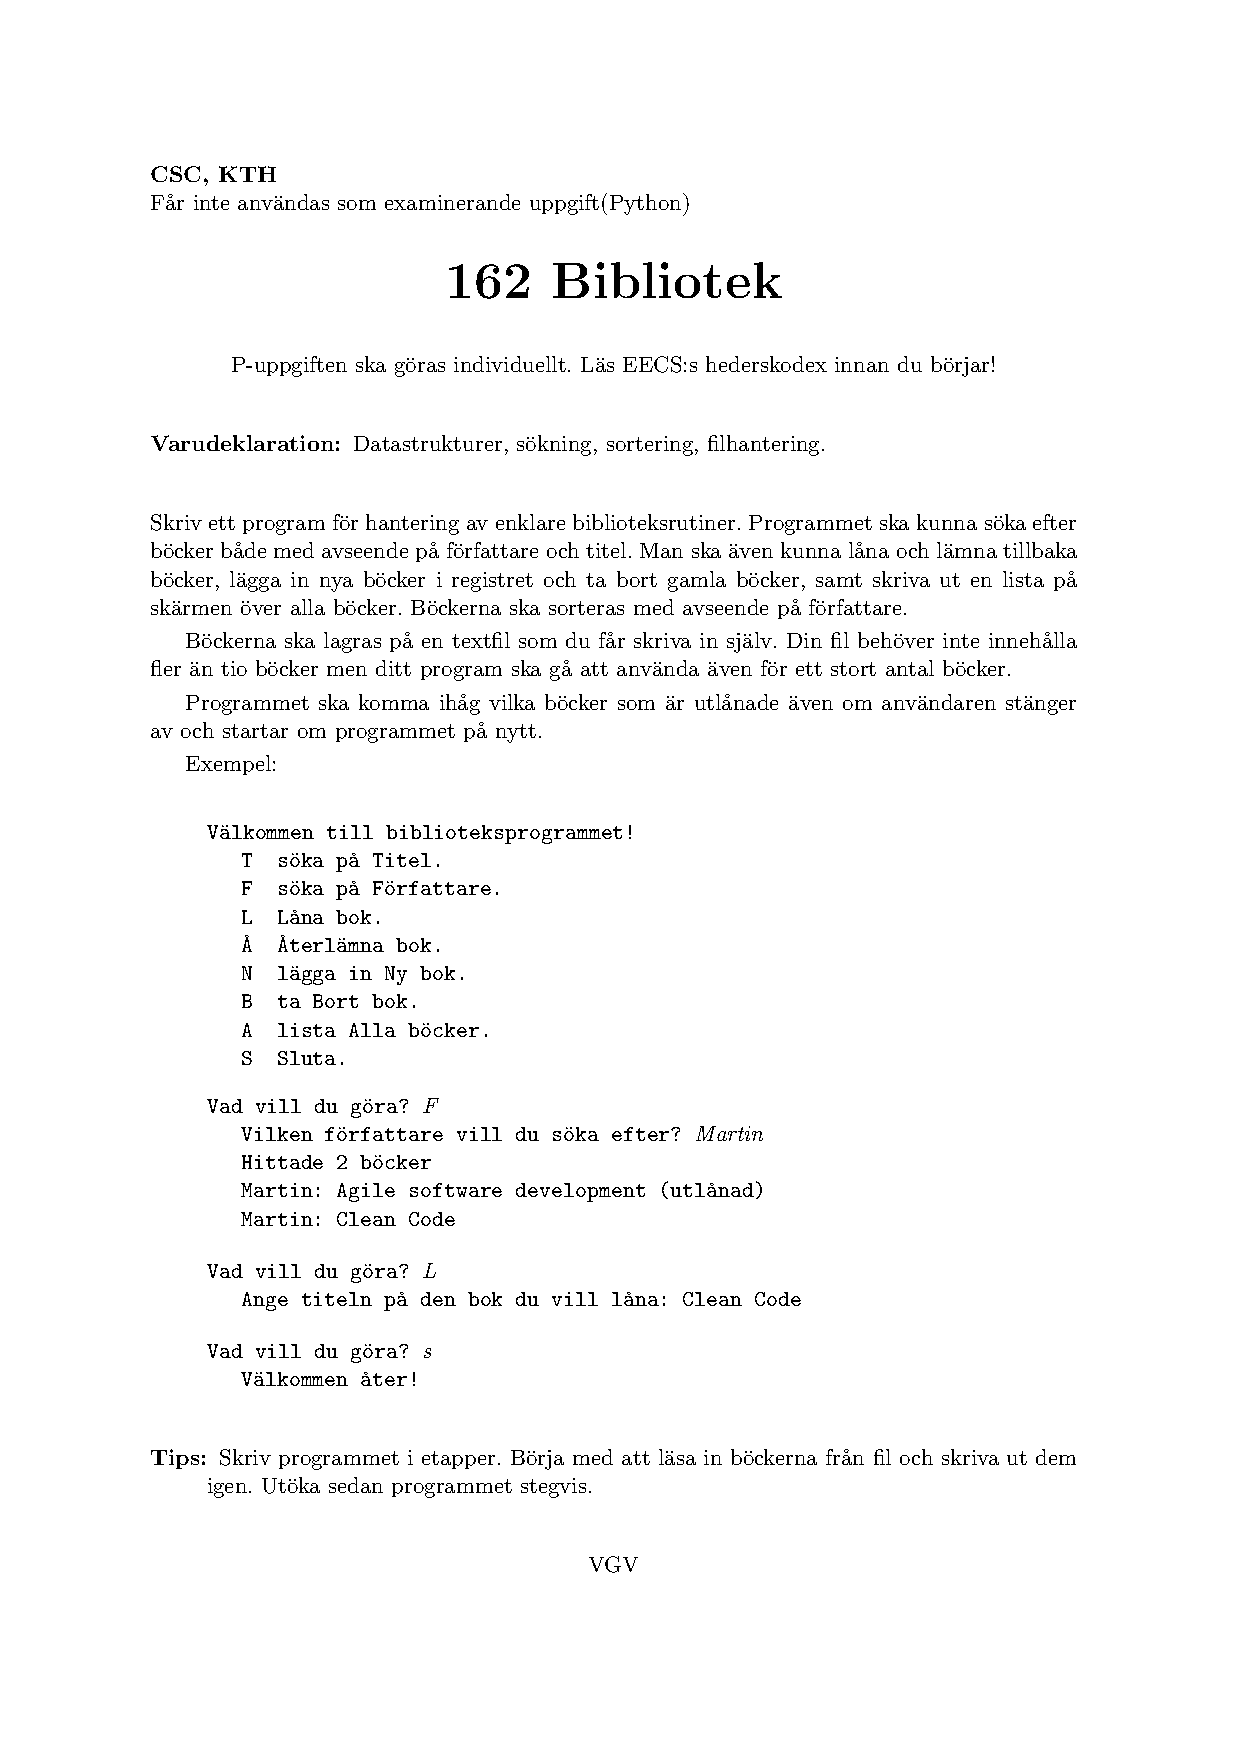
\includegraphics[width=\columnwidth]{exempel.pdf}
\end{frame}


\section{Projektgranskning}

\begin{frame}
  \begin{block}{Granskning}
    \begin{itemize}
      \item Ni ger varandra återkoppling innan redovisningen.
      \item Går igenom samma kriterier som assarna kommer att använda vid 
        redovisning.
      \item \alert{Sikta på att ha projektet klart för granskning 3/12.}
      \end{itemize}
  \end{block}

  \pause

  \begin{remark}
    \begin{itemize}
      \item Det är obligatoriskt att granska, inte att bli granskad.
    \end{itemize}
  \end{remark}
\end{frame}


\section{Projektredovisning}

\begin{frame}
  \begin{block}{Redovisning}
    \begin{itemize}
      \item Projektet är klart.
      \item Ni har fått återkoppling från en annan student.
      \item Nu ska ni presentera för en asse.
      \item Boka tillfällen sista två veckorna innan jul (6--17/12).
      \item \alert{Sikta på att ha projektet granskat och klart senast 10/12.}
    \end{itemize}
  \end{block}

  \pause

  \begin{remark}
    \begin{itemize}
      \item Om behov finns kan vi klämma in några redovisningar efter 
        nyårshelgen.
    \end{itemize}
  \end{remark}
\end{frame}

\begin{frame}
  \begin{block}{Rättningsmatris}
    \begin{itemize}
      \item Samma rättningsmatris som för labbarna.
      \item Ett påpekande \(\implies\) max E i betyg.
      \item Tre påpekanden \(\implies\) F.
    \end{itemize}
  \end{block}
\end{frame}

